\chapter{Safety of Bitcoin}

\section{Introduction}

The security of a blockchain system, such as Bitcoin, is of utmost importance to ensure the integrity and trustworthiness of the network. When analyzing the security of a blockchain, it is crucial to consider the presence of adversaries who may try to disrupt the system for their own gain. In the context of blockchain security, adversaries are often modeled as powerful entities with significant resources, including more information, computational power, and control over the network compared to honest participants.\\
Bitcoin incorporates several security measures to protect honest users from adversarial attacks. These measures include:\\
\textbf{Proof-of-Work Verification:} Honest nodes verify the proof-of-work in new blocks, ensuring that miners have expended sufficient computational effort to create a valid block. This prevents adversaries from easily generating new blocks and taking control of the blockchain.\\
\textbf{Transaction Verification:} Honest nodes validate signed transactions, ensuring that only rightful owners can spend their funds. Transactions that do not follow the rules are ignored.\\
\textbf{UTXO Validation:} Honest nodes keep track of the unspent transaction outputs (UTXOs) and verify that each transaction's inputs reference valid UTXOs. Invalid transactions are not accepted.\\
While these sanity checks are straightforward and easy for honest participants to perform, attacks at the level of the Nakamoto consensus protocol, which determines the longest chain and the agreed-upon version of the blockchain, are more complex and subtle. Adversaries can attempt to disrupt the consensus protocol in ways that are not immediately evident to honest players.\\
Formal mathematical models are used to analyze the security of the Nakamoto consensus protocol. These models treat the mining process as a stochastic process, where new blocks are generated at random intervals of time. The use of stochastic modeling allows for probabilistic analysis of the protocol's security guarantees. The security guarantees in this context are probabilistic because they depend on the randomness inherent in the mining process.\\
By applying formal mathematical methods and probabilistic analysis, researchers can gain insights into the security properties of the Nakamoto consensus protocol. This includes understanding the likelihood of successful attacks by adversaries and the resilience of the blockchain system to such attacks.

\section{Mining as a Poisson process}
A Poisson process is a stochastic process where events occur at random intervals, following the exponential distribution. In this case, the events correspond to the mining of new blocks. The intervals between any two block arrivals are statistically identical and independent of each other.\\
If we denote the time between consecutive block arrivals as X, then X follows an exponential distribution with parameter $\lambda$. The probability that the time between two block arrivals is greater than or equal to t is given by:\\
$$ P(X \geq t) = e^{-\lambda t} \quad \text{for all } t \geq 0. $$

This probability is often used to analyze the behavior of the Poisson process and to estimate the time it takes for the next block to be mined, given the current rate $\lambda$. The exponential distribution is particularly useful in modeling Poisson processes, as it captures the randomness and memorylessness properties of the arrival times in the process.\\
Indeed, a Poisson random variable Y with parameter $\lambda$ has a probability mass function given by:
$$P(Y = k) = \frac{e^{-\lambda} \lambda^k}{k!} \quad \text{for all } k \geq 0.$$
In a Poisson process, the number of events (block arrivals in this case) in an interval of length $T$ follows a Poisson distribution with parameter $\lambda$T, assuming the average rate  $\lambda$ remains constant. Furthermore, the number of events in disjoint intervals of time is statistically independent.\\
If we consider small intervals of time ($\lambda T << 1$), the probability of having one event (block mined) in the interval is approximately  $\lambda T$, and the probability of having no events (no block mined) is approximately $1 - \lambda T$. This approximation is justified because $\lambda T$ is very small, given the average rate $\lambda$ is generally small when expressed in terms of the number of blocks per unit of time.\\
This is where the analogy with coin tosses comes in. A Poisson process can be emulated by counting the occurrence of "successes" (in this case, block arrivals) in a sequence of independent Bernoulli trials (coin tosses), where the probability of success (head) is very small (approximately equal to $\lambda T$).\\
In modeling the mining process as a Poisson process, we assume that the total number of hashes computed (or nonces tried out) per unit of time remains roughly constant, even if the number of miners and their individual computation power may vary. This assumption allows us to treat the mining process as a random process, where new blocks are found at random intervals.\\
Let's recap some important modeling assumptions about the mining process in the context of the Nakamoto consensus protocol:\\
\begin{enumerate}
    \item \textbf{Constant Mining Rate ($\lambda$):} We assume that the mining rate (the average number of blocks mined per unit time) is a constant, denoted by  $\lambda$. In Bitcoin, the average block time is about 10 minutes, so  $\lambda$ is approximately 1 block every 600 seconds. In Ethereum, the block time is much faster, so the value of  $\lambda$ is higher.
    \item \textbf{Poisson Process:} The mining process is modeled as a Poisson process, where new blocks are found at random intervals following an exponential distribution. The Poisson process assumption holds because the probability of successfully mining a block in a given second is very small (0.03 in the example given), and the mining process is essentially like flipping a biased coin (trying out nonces) repeatedly, where each flip is independent of the others.
    \item \textbf{Independent and Constant Difficulty:} We assume that the difficulty level of the hash puzzle for proposing a block remains constant over some period of time. The difficulty level determines the number of leading zeros required in the hash output, and a high difficulty makes finding a valid block more challenging. In reality, the difficulty is adjusted regularly to maintain a constant mining rate, and this ensures that the time to mine a block remains relatively constant over time.
    \item \textbf{Uniform Distribution of Valid Nonces:} Valid nonces (hash inputs) are assumed to be uniformly distributed among all possible nonces. This is a common assumption in modeling proof-of-work systems like Bitcoin.
    \item \textbf{Idealized Network and Synchronization:} The model assumes an idealized network where all nodes receive blocks and transactions immediately, and there are no network delays or partitions. In practice, real-world networks introduce latency and possible partitions, affecting block propagation and communication.
    \item \textbf{Honest Majority:}  We assume that the majority of miners in the network are honest, following the protocol correctly. This is a common assumption in security analysis, as most blockchain systems rely on the assumption that a majority of computational power is controlled by honest participants.
\end{enumerate}
By making some of these modeling assumptions and giving the adversary some extra power, the security analysis can provide guarantees that hold even in practical scenarios where real-world considerations might deviate from the idealized assumptions. The goal is to design a protocol that remains secure and resilient in the face of adversarial attacks, even when the adversary has considerable computational power and control over the network.

\section{Nakamoto consensus protocol model}
In the model, we assume the presence of a single adversary with a fraction of the total computing power (hash power) denoted by $\beta$. The remaining computing power, $1 - \beta$, is distributed roughly equally among the many honest parties participating in the protocol.\\
To be more precise:
\begin{itemize}
    \item The adversary's computing power is $\beta$ times the total computing power of all users in the system.
    \item The computing power of honest users is divided equally among them, with each honest user controlling a very small fraction $\frac{1 - \beta}{N}$, where $N$ is the total number of honest users. 
\end{itemize}
This means that the adversary mines blocks at a rate of $\beta \lambda$ (Poisson process of rate $\beta \lambda$), while honest users mine blocks at a combined rate of $(1 - \beta)\lambda$ (Poisson process of rate $(1 - \beta)\lambda)$. The processes of the adversary and the honest users are independent of each other.\\
This assumption gives the adversary a significant advantage in terms of mining power, as it controls a substantial portion of the total computing power. The adversary's higher mining rate $(\beta\lambda)$ compared to that of honest users $((1 - \beta)\lambda)$ allows them to have a higher probability of finding new blocks and building their own chain. However, we still assume that $\beta < \frac{1}{2}$, which means that the honest users collectively have more mining power than the adversary. This assumption is crucial to ensure that the Nakamoto consensus protocol remains secure even in the presence of an adversary.\\
In the model, we assume that each honest player (party) stores a single blockchain at all times, which is the longest chain they have heard until that specific time. Let's denote the chain held by party h at time i as $C_{i}^{h}$.\\
Here's a more detailed explanation of the notation:\\
\begin{itemize}
    \item i $\in$ R+: This represents a continuous-time parameter, which denotes the specific point in time during the protocol execution. The time parameter i can take any non-negative real value.
    \item $C_{i}^{h}$: This notation represents the chain held by party h at time i. The chain $C_{i}^{h}$ is a sequence of blocks, starting from the genesis block (the first block) up to the last block at time i that party h has seen and believes to be part of the longest chain.
\end{itemize}
In this model, honest players continuously update their chain to be the longest chain they have seen so far. This implies that if a party hears of a new block that extends the current longest chain, they update their chain accordingly to include this new block. As a result, the chain $C_{i}^{h}$ held by each honest party h may vary over time as new blocks are discovered and added to the blockchain.\\
The longest chain rule states that honest players always work on extending the longest chain they know, assuming it is the valid chain. As more blocks are mined and added to the blockchain, the chain held by each honest party h ($C_{i}^{h}$) keeps growing as they update it to follow the longest chain.\\
In the model, when an honest party hears of multiple chains with the same (maximum) length, they choose one of them arbitrarily as $C_{i}^{h}$. This choice is made by the adversary, which means that an honest user may swap its chain when it hears of an equally long chain, not just a strictly longer one. Additionally, if two honest parties both hear of two chains of equal (maximum) length, they may adopt different chains due to this arbitrary tie-breaking power given to the adversary.\\
To define the notion of the prefix of a chain, we say that chain C1 is a prefix of chain C2 if all blocks in C1 are also present in C2. Formally, we denote this by C1 $\leq$ C2. To represent the prefix of a chain, we use the notation $C^{h^{⌊}}$, which represents the prefix chain obtained by dropping the last k blocks from chain C. If chain C has less than or equal to k blocks, C⌊k will be considered as the genesis block.\\
The k-deep confirmation rule in Bitcoin implies that a node treats all but the last k blocks in its longest chain as confirmed. In the notation of the model, the blocks in $C^{h^{⌊}}$ are confirmed by user h at time i. Once we confirm a block, we also confirm all the transactions in it. The confirmation rule is applied locally by each user, which means that a transaction confirmed by one user may not be confirmed by another. However, it is desirable that a transaction confirmed by one user becomes confirmed by all other users relatively quickly and remains confirmed forever after. This desirable property is called a safety property in blockchains.\\
In the context of safety, it is important to ensure that once a block is confirmed (included in the longest chain) by a significant number of honest parties, it is highly unlikely to be reversed or replaced by another chain. In other words, a confirmed block's position in the blockchain should be secure and unlikely to be changed. This property is crucial for maintaining the consistency and integrity of the blockchain, especially in the presence of adversarial behavior. Ensuring safety is an essential aspect of blockchain protocols to maintain the trust and reliability of the system.
\section{Formal definitions of safety}
In the Nakamoto consensus protocol, safety is a crucial property that ensures the consistency and integrity of the blockchain. We define safety in two different ways: the common prefix property and individual block safety.\\
\textbf{Definition 1 (Common Prefix Property):}\\
The k-common prefix property holds during the execution of the protocol if any block that is committed by one honest user appears in every honest user's chain thereafter. In mathematical terms, for all pairs of times $i_{1}$ $\leq$ $i_{2}$ and for all pairs of honest users $h_{1}$, $h_{2}$:
$C^{⌊^{k}} \leq C_{2}$,
where $C_{1} \equiv	 C_{i_{1}}^{h^{1}} and C_{1} \equiv C_{i_{2}}^{h^{2}}.$\\
Definition 2 (Individual Block Safety):
In an execution, a block B present in some honest user's chain is safe if, after it has been committed by any honest user, it remains a part of all honest users' chains. In mathematical terms, if block B is committed by some user h at time t, then for all $t′ \geq t$ and for all honest users $h′$, $B \in C_{t'}^{h′}$.\\
Note that the common prefix property subsumes individual block safety. For simplicity, the focus is on individual block safety alone.\\
These definitions represent the desired security properties of the protocol. To ascertain whether such properties hold or with what probability they hold, further calculations and analysis are required. Security guarantees or theorems are typically given with the form that the $k$-common prefix property holds with a probability approaching one as $k$ approaches infinity. These guarantees are made under specific assumptions, including a fixed mining rate, bounds on the adversary's computing power, and bounds on network delays. Importantly, these guarantees are provided while assuming that the adversary can act arbitrarily, meaning no specific assumptions are made about the adversary's strategy.\\
To understand how the adversary can disrupt safety, it is essential to consider possible adversarial actions. In particular, the focus is on an adversary attempting to disrupt the individual safety of a specific block B. By understanding the various strategies the adversary can employ, a comprehensive analysis of the protocol's security can be performed.
\section{Private attack}
In the simple model of the blockchain system with one adversarial user and many honest users, the adversary aims to violate the safety of a specific block B by performing a private attack. The adversary's goal is to first confirm block B by some (or all) honest users and then dislodge it from the longest chain in the future.\\
One possible attack is the private attack, previously introduced in Lecture 3. Here's a more detailed description of the attack:
\begin{enumerate}
    \item The adversary identifies block B's parent, denoted as $B′$, and immediately mines a conflicting block on $B′$ right after $B′$ is mined. The adversary continues mining privately, extending this hidden chain. 
    \item Meanwhile, the honest users, unaware of the private chain, continue mining on the longest chain below block $B$.
    \item The honest and adversarial chains are independent of each other and follow Poisson processes with rates $(1 − \beta)\lambda$ and $\beta\lambda$, respectively. (Recall that $\beta$ represents the fraction of hash power controlled by the adversary.)
\end{enumerate}
To successfully perform the private attack and violate the safety of block $B$, the adversary must reveal its private chain at the right time. If the adversary reveals the private chain while it is still shorter than the longest honest chain, the honest users will simply ignore the adversary's chain, and the attack will have no effect.\\
Therefore, the adversary must wait until its private chain is at least as long as the honest chain containing block $B$ (see Figure \ref{fig:f1}). This way, when the adversary reveals its chain, it will create a fork from a block preceding $B$ and eventually produce a chain of equal or longer length than the longest chain containing $B$.\\
Timing is critical for the success of the private attack. If the adversary reveals its chain too early, even if it displaces block $B$, the attack will not lead to a safety violation. The adversary must wait until the honest chain is long enough, at least $k$ deep, for the attack to have the desired impact and violate the safety of block $B$. 
\begin{figure}[h!]
    \centering
    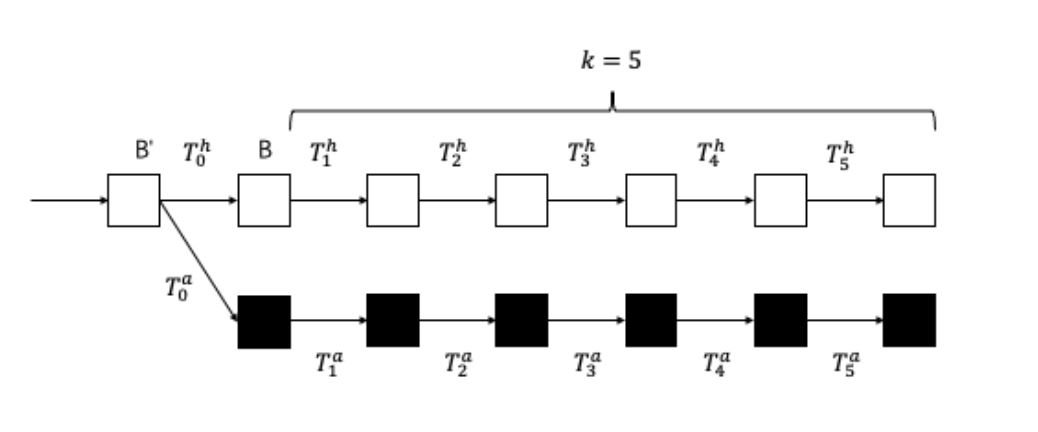
\includegraphics[width=0.6\linewidth]{Fig/06/F1}
    \caption{Private attack on block $B$ with $k = 5$.}
    \label{fig:f1}
\end{figure}
\section{Analysis of the private attack under zero delay}
Suppose now that the network delay $\delta = 0$. So any node mined successfully by an honest node reaches all other nodes instantaneously. One immediate effect of this is that the honest nodes always have access to the latest mined block and thus can always mine on the tip of the longest public blockchain (by potentially switching their mining upon receiving a new block). Denote the time intervals between the honest and adversarial blocks in the chains of length $k + 1$, following block $B′$ by ($T_{0}^{h}, T_{1}^{h}, . . . T_{k}^{h}$) and ($T_{0}^{a}, T_{1}^{a}, . . . T_{k}^{a}$) respectively (see Figure \ref{fig:f1}, where $k = 5$). Then the private attack is successful exactly when the total time to mine $k + 1$ blocks by the adversary is faster than the time the honest miners take to mine their $k + 1$ blocks, i.e.,
\begin{equation*}
    \sum_{i=0}^{k} T_{i}^{h} \geq \sum_{i=0}^{k} T_{i}^{a}
\end{equation*}
Note that the times are all independent of each other and $T_{0}{h}, . . . , T_{k}{h}$ are identically distributed as exponential random variables with mean $(\frac{1}{1 - \beta\lambda})$ and $T_{0}^{a}, . . . , T_{k}^{a}$ are identically distributed as exponential random variables with mean $\frac{1}{\beta\lambda}$. By the law of large 
numbers
\begin{equation*}
    \frac{1}{k + 1}\sum_{i=0}^{k} T_{i}^{h} - T_{i}^{a}   -> \frac{1}{(1 - \beta) \lambda} - \frac{1}{\beta\lambda}.
\end{equation*}
The limiting value is positive (i.e., the private attack is successful) exactly when
\begin{equation*}
    \frac{1}{(1 - \beta) \lambda} > \frac{1}{\beta\lambda}.
\end{equation*}
or simply $\beta > \frac{1}{2}$, i.e., the adversary controls a majority of the hash power. This calculation shows that in the limit of $k$ very large, the safety of any block $B$ in the longest chain of Bitcoin will continue to remain in the longest chain with probability approaching one. In general, there is a tradeoff between a confirmation depth of $k$ and the resulting safety of a block $B$ that has k blocks mined under it. The probability of “de confirmation”, i.e., the block $B$ gets dislodged from the longest chain can be calculated as follows (here $s > 0$ is a parameter to be chosen later):
\begin{equation}
    P(\sum_{i=0}^{k}(T_{i}^{h} - T_{i}^{a}) > 0) = P(s\sum_{i=0}^{k}(T_{i}^{h} - T_{i}^{a}) > 0) = P(e^{s\sum_{t=0}^{k}(T_{i}^{h} - T_{i}^{a})} > 1)    
\end{equation}

\begin{equation}
    \leq E[e^{s\sum_{i=0}^{k}(T_{i}^{h} - T_{i}^{a})}] = E[\prod_{i=0}^{k}e^{s(T_{i}^{h} - T_{i}^{a})}] = \prod_{i=0}^{k}E[e^{s(T_{0}^{h} - T_{0}^{a})}]
\end{equation}

\begin{equation}
     = (\frac{\beta\lambda}{\beta \lambda + s})^{k + 1} (\frac{(1 - \beta) \lambda}{(1 - \beta) \lambda - s})^{k + 1}
\end{equation}

because of the factorization of the moment-generating function of independent random variables. Choosing $s = (1−\frac{2\beta\lambda}{2})$ minimizes the exponent and we see that the probability of deconfirmation of a block $B$ is upper bounded by $e^{−c(k+1)}$ where the exponent is given by:
$c = − \log_{e}(4\beta(1 - \beta)) > 0.$
So the probability of deconfrmation decays exponentially in k, as also illustrated in Figure \ref{fig:f2}. Turns out this calculation was also conducted by Nakamoto themself, albeit somewhat incorrectly, which is included in Figure 2 as a comparison.
\begin{figure}[h!]
    \centering
    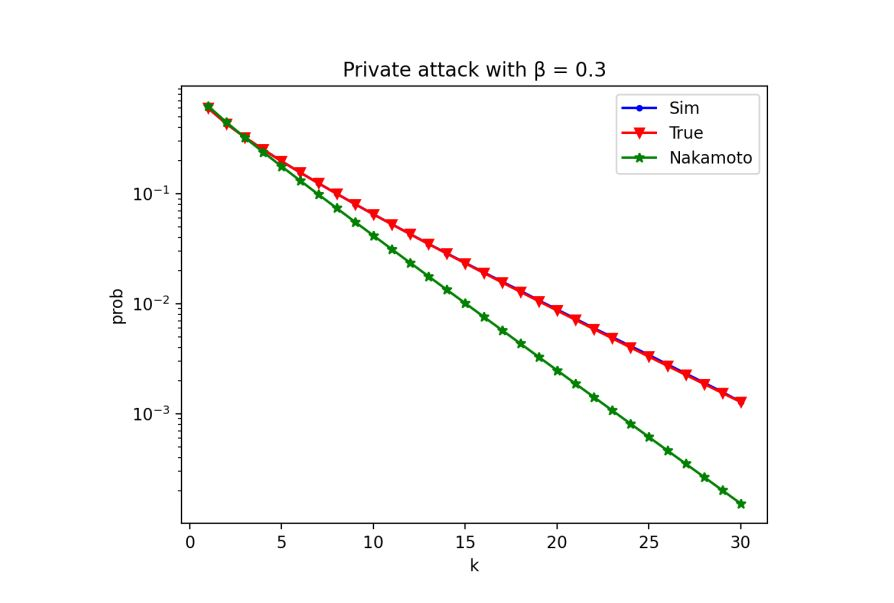
\includegraphics[width=0.6\linewidth]{Fig/06/F2}
    \caption{Private attack with $\beta = 0.3$.}
    \label{fig:f2}
\end{figure}
\section{Private attack is the worst-case attack}
The balance attack is another type of attack on the safety of the blockchain, where the adversary mines and releases blocks in a way that balances the heights of two chains. This prevents any one chain from stabilizing, causing constant switching between the two chains and preventing the ledger from stabilizing.\\
In the case of zero network delay (where all miners instantaneously learn of any newly mined block), it has been observed that whenever any attack on safety is successful, the private attack is also successful. In this context, safety refers to the $k$-deep confirmation rule, which means that blocks deeper than $k$ blocks in the longest chain are considered confirmed. Here are some key observations related to this:
\begin{enumerate}
    \item To launch a safety attack (a balancing attack), at least two chains of length $k + 1$ must be present: one chain to confirm a block $B$ (of depth k) and another chain to de-confirm block B by switching the longest chain.
    \item Therefore, the total number of blocks mined by both the adversary ($A_{k}$) and the honest nodes ($H_{k}$) during the attack must be at least $2k + 2: A_{k} + H_{k} \geq 2k + 2$.
    \item Due to zero network delay, two honest nodes can never mine at the same level of the blockchain. Honest nodes always mine on the tip of the longest chain, preventing parallel mining at the same level.
    \item For two chains to have a length of at least $k + 1$ (to launch the safety attack), the number of adversarially mined blocks must be larger than the number of honest mined blocks: $A_{k} \geq H_{k}$.
\end{enumerate}
From these observations, it follows that $A_{k} \geq k + 1$, which means that the adversary has successfully mined at least $k + 1$ blocks by the time of the safety attack on the $k$-deep confirmation rule.\\
The significance of this result is that, in the case of zero network delay, any attack that successfully violates safety (such as a balance attack) requires the adversary to have already mined at least $k + 1$ blocks. And with this number of blocks, the adversary could have used them to launch a private attack instead.\\
This observation is crucial in understanding the relationship between different attack strategies and provides insights into the security of the Nakamoto consensus protocol under various conditions. It shows that the private attack is a powerful and general attack strategy, and other attacks, like the balance attack, are limited in their effectiveness compared to the private attack (Figure \ref{fig:f3}). 
\begin{figure}[h!]
    \centering
    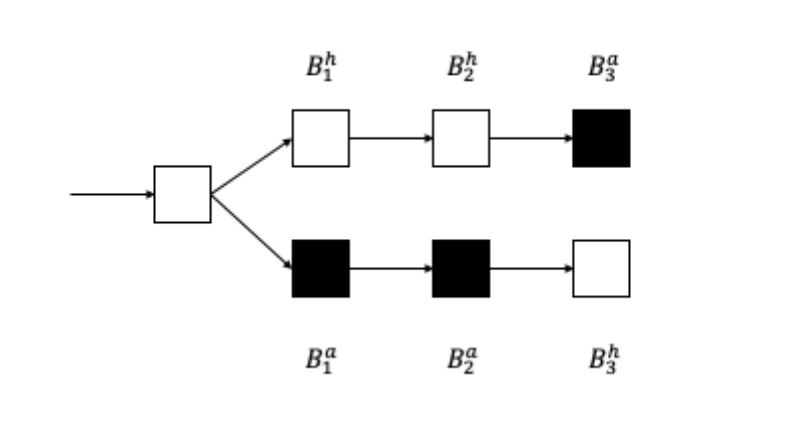
\includegraphics[width=0.6\linewidth]{Fig/06/F3}
    \caption{Illustration of a balance attack.}
    \label{fig:f3}
\end{figure}
\section{Safety analysis under bounded network delay}
In the $\delta$-synchronous network model with propagation delay, there is a finite amount of time $\delta$ within which all blocks reach all participants definitively. The adversary can deliver blocks to different participants at a time of its choosing, as long as the $\delta$-synchrony condition is met. This introduces natural forking in the blockchain, even without adversarial intervention.\\
In the context of Bitcoin, with an inter-block arrival time of ten minutes, natural forking is not very prevalent because it is unlikely that honest nodes will mine on stale blocks. However, in other blockchains like Ethereum, where the inter-block arrival time is fourteen seconds, natural forking is more common due to the shorter block time.\\
The term $(1 - \beta)\lambda\delta$ represents the expected number of blocks that are being mined "in parallel" by the honest nodes. Here, $(1 - \beta)\lambda$ is the rate at which honest blocks are mined, and $\delta$ is the network delay. This means that during the time $\lambda$, the honest nodes may mine multiple blocks, but only one of these blocks will succeed in extending the longest chain. The other blocks mined in parallel are considered "wasted" because they will not become part of the final longest chain.\\
For example, if the honest fraction of hash power $(1 - \beta)\lambda$ is $0.9$ and the network delay $\delta$ is $10$ seconds, then the expected number of parallel blocks mined by honest nodes during this time is $0.9$ blocks. Out of these $0.9$ blocks, only one block will eventually be included in the longest chain, and the remaining $0.9 - 1 = -0.1$ block is considered a "wasted" mining effort.\\
In blockchains with shorter block times and higher natural forking rates, a larger fraction of honest mining power may be "wasted" due to natural forking. This natural forking phenomenon is an inherent characteristic of the Nakamoto consensus protocol in blockchain systems and affects the efficiency of the mining process.\\
Thus the rate of growth of the honest chain is now reduced by a fraction $\frac{1}{1+(1 - \beta)\lambda\delta}$ to
\begin{equation*}
    \frac{(1 - \beta) \lambda}{1 + (1 - \beta) \lambda \beta}
\end{equation*}
Now an adversary launching a private attack is successful if its rate of growth (of a private chain) is larger than that of the (reduced) growth rate of the honest chain:
\begin{equation}
    \beta \lambda > \frac{(1 - \beta) \lambda}{1 + (1 - \beta) \lambda \beta}
\end{equation}
\begin{figure}[h!]
    \centering
    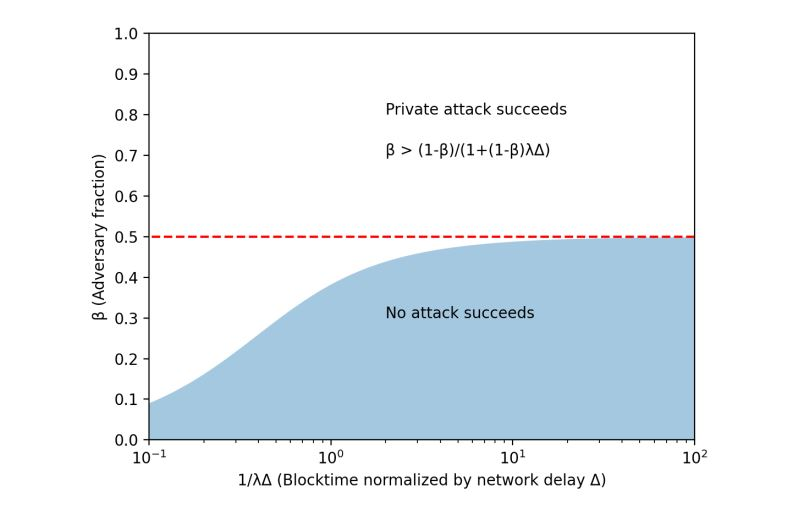
\includegraphics[width=0.6\linewidth]{Fig/06/F4}
    \caption{Minimum hash power needed by the adversary to succeed in its private attack. It turns
        out that this is also the security threshold for the adversary to successfully launch any safety attack.}
    \label{fig:f4}
\end{figure}
Figure \ref{fig:f4} illustrates the minimum hash power the adversary needs to succeed in its private attack, i.e., to replace a certain number of blocks on the longest chain with its own longer chain. The adversary can execute the private attack by mining blocks in secret and then revealing them at a strategic moment to create a longer chain that overtakes the honest chain.\\
Previously, we saw that when the network delay ($\delta$) is zero, the private attack is a worst-case attack in a very general setting. This means that for every sample path of the mining process and for every confirmation depth ($k$), the private attack is successful whenever any attack is successful. However, in cases where the network delay is non-zero ($\delta > 0$), the private attack may not always be the worst-case attack.\\
Figure \ref{fig:f5} shows an example where the private attack is not the worst-case attack. In this scenario, the adversary can use a different strategy and still succeed in disrupting the safety of the blockchain, even though the private attack fails. This implies that the private attack is not always the most effective attack in the presence of network delay.\\
However, despite this, it turns out that the private attack is still a worst-case attack in the sense of the minimum required honest hash power to ensure safety against all attacks. In other words, if the blockchain system can withstand the private attack with a certain level of honest hash power, it can also withstand any other attack with the same level of honest hash power. This safety guarantee holds with probability approaching one as the confirmation depth ($k$) approaches infinity.\\
The reason why the private attack is still a worst-case attack in terms of the required honest hash power is due to the inherent properties of the Nakamoto consensus protocol. The protocol is designed such that an attacker needs to have a majority of the total hash power to overpower the honest nodes and control the longest chain. Therefore, the same condition derived for the success of the private attack also holds for any other attack, and the private attack remains a worst-case scenario for determining the minimum required honest hash power to ensure safety in the blockchain system.
\begin{figure}[h!]
    \centering
    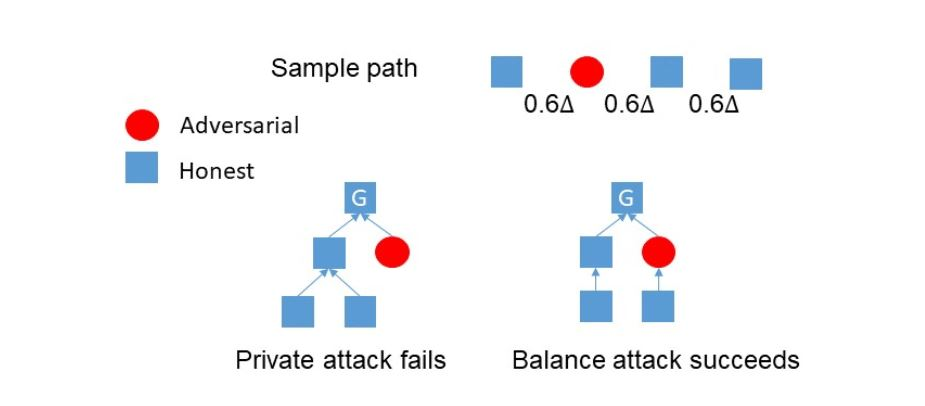
\includegraphics[width=0.6\linewidth]{Fig/06/F5}
    \caption{Attacks aimed to create a fork with length 2}
    \label{fig:f5}
\end{figure}
\begin{figure}[h!]
    \centering
    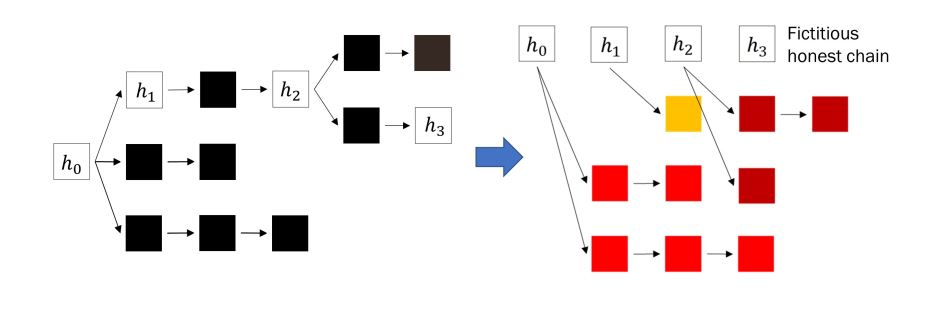
\includegraphics[width=0.6\linewidth]{Fig/06/F6}
    \caption{By block tree partitioning, a general attack is represented as multiple adversarial chains simultaneously racing with a fictitious honest chain. Note that this fictitious chain is formed by only the honest blocks, and may not correspond to the longest chain in the actual system. However, the longest chain in the actual system must grow no slower than this fictitious chain.}
    \label{fig:f6}
\end{figure}

\section{Nakamoto blocks}
The analysis of attacks on the blockchain system becomes more complicated when the network delay ($\delta$) is non-zero, and the entire block tree can be arbitrary due to multiple adversarial actions at different time instances. However, we can still gain insights by partitioning the complex block tree into subtrees, each rooted at an honest block and consisting entirely of adversarial blocks (public or private).\\
By doing this, we can view the general attack as initiating multiple adversarial subtrees that race with a single fictitious chain consisting of only honest blocks (Figure \ref{fig:f6}). Each adversarial subtree's growth rate is upper-bounded by the growth rate of the adversarial chain used in the private attack. Therefore, if the private attack is unsuccessful, we know that the growth rate of each adversarial subtree must be less than that of the fictitious honest chain.\\
Under this condition, there must exist honest blocks, referred to as Nakamoto blocks, that have the special property that none of the past adversarial subtrees can ever catch up to the honest chain after the honest chain reaches that particular block (Figure \ref{fig:f7}). These Nakamoto blocks play a crucial role in stabilizing the blockchain. When a Nakamoto block occurs and occurs frequently, it guarantees the safety of the protocol.\\
The presence of Nakamoto blocks ensures that the prefix of the longest chain up to that block remains immutable in the future. In other words, once a Nakamoto block is included in the blockchain, it becomes a solid anchor that protects the entire prefix of the longest chain before that block from any adversarial reorganization attempts. This stability ensures that the blockchain system maintains its safety guarantees, and honest users can have confidence in the integrity of the ledger.\\
When Nakamoto blocks occur regularly, the blockchain's safety is effectively guaranteed, even in the presence of adversarial attacks. The analysis helps us understand how certain key blocks in the blockchain, such as Nakamoto blocks, play a critical role in maintaining the system's security and ensuring that honest users' transactions remain protected and valid.

\begin{figure}[h!]
    \centering
    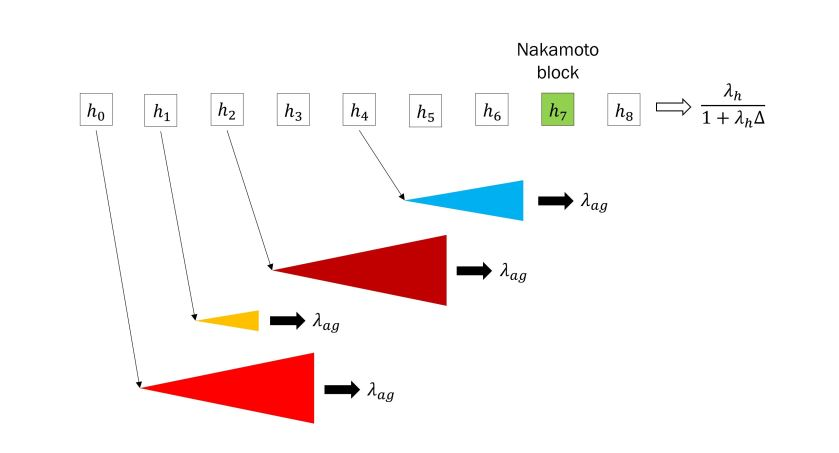
\includegraphics[width=0.6\linewidth]{Fig/06/F7}
    \caption{Race between the adversarial trees and the fictitious honest chain. While there may be multiple adversarial trees simultaneously racing with the honest chain, the growth rate of each tree is bounded by the growth rate of the adversarial chain in the private attack. An honest block is a Nakamoto block when all the previous adversarial trees never catch up with the honest chain past that block. To simplify notations, $\lambda_{ag} = \beta\lambda$ and $\lambda h = (1 − \beta)\lambda$.}
    \label{fig:f7}
\end{figure}

\section{Importance of synchronous network}
The safety analysis of the longest chain protocol in this lecture highlights the importance of keeping the adversarial hash power within certain bounds relative to the overall mining rate and worst-case network delay. As long as the adversarial hash power is limited, the protocol remains safe, ensuring that the blockchain maintains its integrity and security.\\
However, the analysis also emphasizes the significance of having a finite worst-case network delay. In a purely asynchronous network, where there are no guarantees on message delivery times, the adversary can exploit the lack of synchronized communication to break consensus. By mining alternate chains and selectively sharing them with different subsets of honest nodes, the adversary can create confusion and disagreement among the nodes, leading to a breakdown of consensus and safety.\\
To address this issue, an intermediate network scenario, known as the partially synchronous network model, is considered. In this setting, the network delays are finite but unknown. There is a global stabilization time (GST), after which all messages are guaranteed to be delivered to all nodes within a bounded time. In this partially synchronous setting, safety can potentially be violated because the confirmation depth $k$ (used in the $k$-deep confirmation rule) could be smaller than the GST, allowing for vulnerabilities.\\
However, it is crucial to note that after the GST, consensus is restored, and the blockchain system becomes safe once again. This highlights the trade-off between the guarantees of safety and the network conditions in such scenarios.\\
In subsequent lectures, the focus will shift to studying consensus protocols that can ensure safety even under partially synchronous network settings, addressing the challenges posed by the unknown and varying network delays. These protocols aim to provide robustness and security even in more realistic network conditions, ensuring the integrity of the blockchain system under various scenarios.
